\chapter{Laws of Motion, Phase Space, and Conservation}

We begin, as the lecture does, with a wrong law. That is not a historical ornament. It is a test. If a law of motion is supposed to tell us what happens next, and if fundamental laws are supposed to preserve enough structure that the past can in principle be recovered from the present, then Aristotle's law is worth studying precisely because it fails. From that failure we are led, step by step, to Newton's law, to momentum, to phase space, and then to the first serious conservation laws of mechanics.

\section{Aristotle's Law in a Friction-Dominated World}

Aristotle's intuition is not foolish. In a world dominated by friction, it really does look as though motion requires a continuing push: stop pushing, and the object stops. The heavier the object, the harder one must push it to give it a certain velocity; the harder one pushes, the faster it goes. That intuition is summarized by the deliberately wrong law
\begin{equation}
\vec F = m\vec v.
\end{equation}
We write it down not to endorse it, but to see exactly what kind of law it is.

For documentary context, it is worth keeping the original board moment in view.

\begin{figure}
\centering

\includegraphics[width=0.82\textwidth]{lecture_02_figure_02.png}
\end{figure}

In one dimension this becomes
\begin{equation}
F = m\dot x.
\end{equation}
Now the lecture immediately insists on a very important point: a law becomes intelligible only when it can be read as an update rule. So let us discretize time into small steps of size \(\delta\). Then
\begin{equation}
\dot x(t) \approx \frac{x(t+\delta)-x(t)}{\delta},
\end{equation}
and Aristotle's law becomes
\begin{align}
F(t) &= m\,\frac{x(t+\delta)-x(t)}{\delta},\\
x(t+\delta) &= x(t) + \frac{\delta}{m}F(t).
\end{align}
This really is a law of motion in the elementary sense: if we know the position at time \(t\), and if we know the force, then it tells us the position at time \(t+\delta\).

There is already something peculiar here. If \(F=0\), then \(\dot x=0\), so the object does not continue in motion; it simply sits still. Aristotle's law predicts a static past and a static future when the force vanishes. That is already quite unlike Newton, but the deeper defect emerges only when we try an explicit example.

\section{Aristotle's Spring and the Loss of the Past}

Take the simplest force depending on position alone, the spring force,
\begin{equation}
F(x)=-kx.
\end{equation}
Insert this into the Aristotle update rule:
\begin{equation}
x(t+\delta)=x(t)-\frac{k\delta}{m}x(t)
=\left(1-\frac{k\delta}{m}\right)x(t).
\end{equation}
If \(\delta\) is small, then \(1-k\delta/m\) is slightly less than \(1\). Each step multiplies the position by the same constant factor. The position therefore shrinks geometrically toward the origin.

The continuous form makes the point even cleaner:
\begin{equation}
m\dot x=-kx,
\end{equation}
whose solution is
\begin{equation}
x(t)=x(0)e^{-kt/m}.
\end{equation}
So under Aristotle's law the displaced spring does not oscillate. It simply drifts back toward equilibrium, slower and slower, exponentially approaching rest.

\subsection{Question \& Answer}

The lecture naturally pauses here to ask: in what sense does Aristotle's law fail to predict the past?

The answer is not that one cannot formally solve the equation backward if one has infinite precision. The sharper point is that distinct initial conditions collapse onto practically indistinguishable final conditions. Many different starting points all drift into the same resting state at the origin. Once the system has nearly settled there, finite observational accuracy is no longer enough to tell where it came from. The law predicts the future, but it does not preserve distinctions well enough to recover the past in any practical sense. That is the lecture's first serious sign of irreversibility.

\section{Newton's Law, Inertial Frames, and the Meaning of Force}

The lecture now pivots sharply. Aristotle's mistake is not merely that he wrote down the wrong proportionality. The deeper mistake is that force does not produce motion; force changes motion. Friction is itself a force, and in ordinary life what often looks like ``force gives velocity'' is really one force balancing another.

Newton's second law is
\begin{equation}
F=m\ddot x.
\end{equation}
Before using it, however, the lecture makes a brief conceptual stop at inertial frames. The point is not to sink into foundations, but to say the right thing plainly: the law of physics is that there exist frames of reference in which Newton's laws are true. One should not define inertial frames in a circle and leave it at that.

Then comes an operational discussion of force and mass. A spring balance gives meaning to a unit of force. Doubling the number of identical springs doubles the force and doubles the acceleration. Doubling the mass at fixed force halves the acceleration. In this way one gives empirical content to the statement that acceleration is proportional to force and inversely proportional to mass.

Once that is in place, the lecture asks the same question it asked of Aristotle: is Newton's law predictive in the same sense?

\section{Momentum, First-Order Form, and Phase Space}

If we discretize the second derivative, we find
\begin{equation}
\ddot x(t)\approx \frac{x(t+\delta)-2x(t)+x(t-\delta)}{\delta^2}.
\end{equation}
So Newton's law becomes
\begin{equation}
x(t+\delta)=2x(t)-x(t-\delta)+\frac{\delta^2}{m}F(t).
\end{equation}
At first sight this is worse than Aristotle's law. To know the next position, it is not enough to know the present position; we also need past information.

\subsection{Question \& Answer}

If Newton's law is second order, why does it still count as a predictive law of motion?

Because ``knowing everything'' about the state has to mean knowing everything needed to predict the future. Newton's law teaches us that the right state is not position alone. We must specify both position and velocity. Equivalently, we may specify position and momentum. The apparent failure of predictiveness is really a clue that the state space has been chosen too small.

This is the reason for introducing momentum:
\begin{equation}
p=m\dot x.
\end{equation}
With constant mass, Newton's law can be rewritten as
\begin{equation}
\dot p = F.
\end{equation}
The board moment where Susskind rewrites the law this way is worth keeping visible.

\begin{figure}
\centering

\includegraphics[width=0.82\textwidth]{lecture_02_figure_03.png}
\end{figure}

In vector language,
\begin{equation}
\vec F=\frac{d\vec p}{dt}.
\end{equation}
And now the second-order equation has been split into two first-order equations:
\begin{align}
\dot p &= F,\\
\dot x &= \frac{p}{m}.
\end{align}
This is exactly the form the lecture wants us to see. One equation updates the momentum from the force; the other updates the position from the momentum.

Again the board layout is pedagogically useful, because it makes visible the claim that Newton's law should be regarded as two first-order equations for two variables.

\begin{figure}
\centering

\includegraphics[width=0.82\textwidth]{lecture_02_figure_04.png}
\end{figure}

The corresponding initial data are therefore
\begin{equation}
(x,p),
\end{equation}
or equivalently \((x,\dot x)\). The space of such data is phase space. That is the decisive conceptual move of the lecture: classical mechanics is not naturally formulated only in the space of positions. It lives in phase space.

\section{The Newtonian Spring, Oscillation, and Time Reversal}

Now let us return to the same spring problem, but this time with Newton's law:
\begin{equation}
m\ddot x=-kx.
\end{equation}
To simplify the algebra and keep the logic in front of us, let us set \(m=1\) and \(k=1\). Then
\begin{equation}
\ddot x=-x.
\end{equation}
Unlike the Aristotle equation, whose solution was exponential decay, this equation has oscillatory solutions. A convenient form is
\begin{equation}
x(t)=c\cos(t-t_0).
\end{equation}
Differentiating gives
\begin{equation}
p(t)=\dot x(t)=-c\sin(t-t_0),
\end{equation}
where we have used \(p=\dot x\) because \(m=1\).

Now compute
\begin{align}
x^2+p^2
&=c^2\cos^2(t-t_0)+c^2\sin^2(t-t_0)\\
&=c^2.
\end{align}
So the motion in phase space lies on a circle:
\begin{equation}
x^2+p^2=c^2.
\end{equation}
That is the real contrast with Aristotle. Under Newton's law the spring does not collapse to a single resting point. Different initial conditions remain on different cycles. Distinctions are preserved.

The lecture then makes the reversibility point in another language. Under time reversal,
\begin{equation}
t\mapsto -t,\qquad \dot x\mapsto -\dot x,\qquad \ddot x\mapsto \ddot x.
\end{equation}
A first time derivative changes sign, a second time derivative does not. Thus Aristotle's law is not invariant under reversal of time, while Newton's equation is. If we film a Newtonian motion and run the film backward, we obtain another solution of the same equations.

This is also the right place to connect back to the earlier discussion of cycles. Once the motion lies on circles in phase space, we expect a conserved quantity labeling those circles. The lecture next turns to conservation laws explicitly.

\section{Momentum Conservation}

The lecture first disposes of a small point: Newton's first law is really the zero-force special case of the second law. Then it turns to Newton's third law.

Assume a closed system of particles, with no external forces. Let \(\vec F_{ij}\) denote the force on particle \(i\) due to particle \(j\). Newton's third law says
\begin{equation}
\vec F_{ij}=-\vec F_{ji}.
\end{equation}
For each particle we write
\begin{equation}
\dot{\vec p}_i=\sum_{j\ne i}\vec F_{ij}.
\end{equation}
Now sum over all particles:
\begin{equation}
\frac{d}{dt}\sum_i \vec p_i = \sum_i\sum_{j\ne i}\vec F_{ij}.
\end{equation}
Every internal force appears twice on the right-hand side: once as \(\vec F_{ij}\), once as \(\vec F_{ji}\). By Newton's third law the pair cancels. Therefore
\begin{equation}
\frac{d\vec P_{\text{tot}}}{dt}=0,
\end{equation}
where
\begin{equation}
\vec P_{\text{tot}}=\sum_i \vec p_i.
\end{equation}
So total momentum is conserved.

In the lecture this is the first true conservation law to be derived from Newtonian dynamics. Only after that pause does Susskind turn to energy.

\section{Energy, Potential, and Conservative Forces}

We begin in one dimension with a single particle moving under a force that depends only on position:
\begin{equation}
F=F(x).
\end{equation}
In one dimension, provided the force is sufficiently well behaved, we may always write it as the derivative of some function \(V(x)\), up to a conventional minus sign:
\begin{equation}
F(x)=-\frac{dV(x)}{dx}.
\end{equation}
The lecture insists on the geometry here. We should picture the particle moving along the \(x\)-axis while the graph of \(V(x)\) forms a landscape of hills and valleys. The force points toward lower altitude, and its magnitude is controlled by the slope.

Now define the total energy by
\begin{equation}
E=\frac12 m\dot x^2+V(x).
\end{equation}
The board derivation is worth preserving, since it records the live passage from the definition of \(E\) to its vanishing time derivative.

\begin{figure}
\centering

\includegraphics[width=0.82\textwidth]{lecture_02_figure_05.png}
\end{figure}

The derivation is straightforward but central:
\begin{align}
\frac{dE}{dt}
&=\frac{d}{dt}\left(\frac12 m\dot x^2\right)+\frac{dV}{dt}\\
&=m\dot x\,\ddot x+\frac{dV}{dx}\dot x\\
&=\dot x\left(m\ddot x+\frac{dV}{dx}\right).
\end{align}
But Newton's law gives \(m\ddot x=F\), and the potential relation gives \(F=-dV/dx\). Hence the bracket vanishes, so
\begin{equation}
\frac{dE}{dt}=0.
\end{equation}
This is energy conservation in one dimension. The kinetic and potential terms trade off against one another, but their sum is fixed.

For a spring,
\begin{equation}
F=-kx,
\end{equation}
so
\begin{equation}
\frac{dV}{dx}=kx,
\end{equation}
and therefore
\begin{equation}
V(x)=\frac{k}{2}x^2.
\end{equation}
The oscillator energy is then
\begin{equation}
E=\frac12 m\dot x^2+\frac{k}{2}x^2.
\end{equation}
When \(m=k=1\), this becomes
\begin{equation}
E=\frac12(\dot x^2+x^2),
\end{equation}
so the phase-space circles are simply the contours of constant energy.

\subsection{Question \& Answer}

Is every force field the gradient of a potential energy?

In one dimension, for sufficiently nice \(F(x)\), the answer is effectively yes: any such function can be integrated, so one can define \(V(x)\) with \(F=-dV/dx\). But the lecture now makes an important turn. In several dimensions this is no longer automatic. If we are given several independent functions \(F_i(x_1,x_2,x_3)\), there is no mathematical necessity that they arise as partial derivatives of a single scalar \(V\). That is not a theorem of calculus. It is a special physical property of conservative forces.

The corresponding board formula and sketch should therefore be kept together.

\begin{figure}
\centering

\includegraphics[width=0.82\textwidth]{lecture_02_figure_06.png}
\end{figure}

What we would like to write is
\begin{equation}
F_i(\mathbf{x})=-\frac{\partial V(\mathbf{x})}{\partial x_i},
\end{equation}
or, in compact form,
\begin{equation}
\vec F=-\nabla V.
\end{equation}
The lecture's contour-map picture makes the meaning of this equation geometrically transparent: the level curves of \(V\) are contours of equal potential, and the force points in the direction of steepest descent, normal to those contours.

A schematic version of that picture is useful to keep beside the board image.

\begin{figure}
\centering
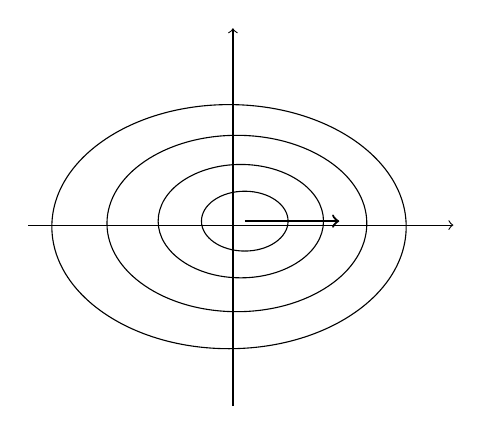
\begin{tikzpicture}[scale=1.0]
\draw[->] (-2.6,0) -- (2.8,0);
\draw[->] (0,-2.3) -- (0,2.5);
\draw (0.15,0.05) ellipse (0.55 and 0.38);
\draw (0.10,0.05) ellipse (1.05 and 0.72);
\draw (0.05,0.02) ellipse (1.65 and 1.12);
\draw (-0.05,-0.02) ellipse (2.25 and 1.55);
\draw[->,line width=0.8pt] (0.15,0.05) -- (1.35,0.05);
\end{tikzpicture}
\end{figure}

Once we assume this conservative-force form, the multidimensional energy is
\begin{equation}
E=\frac12 m\sum_i \dot x_i^2+V(x_1,\dots,x_n).
\end{equation}
Its time derivative is
\begin{align}
\frac{dE}{dt}
&=m\sum_i \dot x_i\ddot x_i+\sum_i \frac{\partial V}{\partial x_i}\dot x_i\\
&=\sum_i \dot x_i\left(m\ddot x_i+\frac{\partial V}{\partial x_i}\right).
\end{align}
If \(F_i=-\partial V/\partial x_i\) and \(m\ddot x_i=F_i\), each bracket vanishes, so again
\begin{equation}
\frac{dE}{dt}=0.
\end{equation}

The many-particle extension is then conceptually unchanged. We flatten all coordinates into a list \(x_1,\dots,x_{3N}\), allow masses \(m_i\), assume a potential \(V(x_1,\dots,x_{3N})\), and define
\begin{equation}
E=\sum_{i=1}^{3N}\frac12 m_i\dot x_i^2+V(x_1,\dots,x_{3N}).
\end{equation}
Under the conservative-force assumption,
\begin{equation}
F_i=-\frac{\partial V}{\partial x_i},
\end{equation}
the same derivation shows that the total energy of the full system is conserved.

\section{Summary}

The lecture has a very tight arc. Aristotle's law was useful because it let us see what a law of motion must do, and what can go wrong when distinct initial conditions collapse onto the same final state. Newton's law repaired that failure, but only after we enlarged the state space from position alone to phase space \((x,p)\). In that language the harmonic oscillator became the simplest example of reversible motion: trajectories move on cycles rather than decaying to a point.

From there the conservation laws followed naturally. Newton's third law gave momentum conservation for a closed system. The existence of a potential gave energy conservation. In one dimension that potential description is almost automatic; in several dimensions it becomes a genuine physical assumption, the assumption that the forces are conservative. With that, the lecture has prepared the ground for the next formulation of mechanics: least action, Lagrangians, Hamiltonians, and the deeper structure that lies beyond Newton's original equations.